\documentclass{article}
\usepackage[utf8]{inputenc}
\usepackage{geometry}
\usepackage{graphicx}
\usepackage{pgfplots}
\usepackage{amsmath}
\usepackage{amssymb}
\usepackage{amsfonts}
\usepackage{mdframed}
\usepackage{amsthm}
\usepackage{physics}
\usepackage{derivative}
\usepackage{hyperref}
\usepackage{wrapfig}
\usepackage{amsthm}
\renewcommand{\theenumi}{\roman{enumi}}

\geometry{a4paper, left=2cm, right=2cm, top=1cm, bottom=2cm}

\pgfplotsset{compat=1.18}
\begin{document}

\begin{minipage}{0.7\textwidth}
    \small \textbf{VARIABLE COMPLEJA}  \\
    \small {Facultad de Ciencias, Universidad Nacional Autónoma de México} \\
    \small {Profesora: Jessie Diana Pontigo Herrera} \\
    \small {Fecha de entrega: 23 de Noviembre de 2024} \\
    \small {Nombre completo: Andrés López González} \\
    \small {Última tarea}
\end{minipage}
\hfill
\begin{minipage}{0.12\textwidth}
    
\includegraphics[width=\linewidth]{logo_universidad}
\end{minipage}

\begin{figure}[h]
    \centering
    
\includegraphics[width=0.9\linewidth]{1.png}
    \label{fig:enter-label}
\end{figure}

\begin{proof}

Considérense las hipótesis
\begin{itemize}
    \item Una función entera \( f(z) \) es una función analítica en todo el plano complejo \( \mathbb{C} \).
   \item Nuestro objetivo es demostrar que si \( f \) está acotada por \( M|z|^n \) fuera del disco \( |z| < \rho \), entonces \( f \) debe ser un polinomio de grado a lo más \( n \).
\end{itemize}

   Esto implica que los coeficientes de \( f \) asociados a \( z^k \) son nulos para \( k > n \) en su expansión en series de potencias. Dado que \( f(z) \) es una función entera, su expansión en serie de potencias alrededor de \( z = 0 \) converge en todo el plano:
   \[
   f(z) = \sum_{k=0}^\infty a_k z^k,
   \]
   donde los coeficientes están dados por la fórmula integral de Cauchy:
   \[
   a_k = \frac{1}{2\pi i} \int_{|z|=R} \frac{f(z)}{z^{k+1}} \, dz.
   \]

   Aquí, \( R > 0 \) es el radio del círculo de integración. Utilizaremos el crecimiento de \( f(z) \) para analizar estos coeficientes; según la hipótesis, para \( |z| \geq \rho \),
   \[
   |f(z)| \leq M |z|^n.
   \]

   En particular, si \( R \geq \rho \), sobre el círculo \( |z| = R \),
   \[
   |f(z)| \leq M R^n.
   \]

   Sustituyendo esta cota en la fórmula para \( a_k \), obtenemos:
   \[
   |a_k| = \left| \frac{1}{2\pi i} \int_{|z|=R} \frac{f(z)}{z^{k+1}} \, dz \right| \leq \frac{1}{2\pi} \int_{|z|=R} \frac{|f(z)|}{|z|^{k+1}} \, |dz|.
   \]

   Como \( |f(z)| \leq M R^n \) y \( |z| = R \), tenemos:
   \[
   |a_k| \leq \frac{1}{2\pi} \int_{|z|=R} \frac{M R^n}{R^{k+1}} \, |dz|.
   \]

   La longitud del círculo \( |z| = R \) es \( 2\pi R \), por lo que:
   \[
   |a_k| \leq \frac{1}{2\pi} \cdot M R^n \cdot \frac{1}{R^{k+1}} \cdot 2\pi R = M R^{n-k}.
   \]

   Si \( k > n \), entonces \( n - k < 0 \), y por lo tanto \( R^{n-k} \to 0 \) cuando \( R \to \infty \). Esto implica que:
   \[
   |a_k| \to 0 \quad \text{para todo } k > n.
   \]

   Dado que \( |a_k| \) es independiente del valor de \( R \), concluimos que \( a_k = 0 \) para todo \( k > n \). Y recapitulando, como los coeficientes \( a_k \) son nulos para \( k > n \), la serie de potencias de \( f(z) \) se reduce a un polinomio de grado a lo más \( n \):
   \[
   f(z) = \sum_{k=0}^n a_k z^k.
   \]
\end{proof}

\begin{figure}[h]
    \centering
    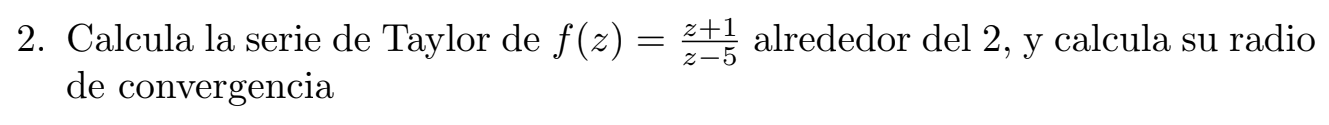
\includegraphics[width=0.8\linewidth]{2.png}
    \label{fig:enter-label}
\end{figure}

\begin{proof}
La función \( f(z) = \frac{z+1}{z-5} \) tiene una singularidad en \( z = 5 \), lo cual será relevante para el cálculo del radio de convergencia, aunque visualmente es directo saber que es 3 por el truquito visto en clase. Expandimos \( f(z) \) en términos de \( w = z - 2 \), con \( z = w + 2 \). Sustituyendo \( z = w + 2 \) en \( f(z) \), obtenemos:
\[
f(z) = f(w+2) = \frac{(w+2)+1}{(w+2)-5}.
\]

Simplifiquemos el numerador y el denominador:
\[
f(w+2) = \frac{w+3}{w-3}.
\]

Así, \( f(z) \) en términos de \( w \) es:
\[
f(z) = \frac{w+3}{w-3}.
\]

Escribimos la expresión como:
\[
f(z) = \frac{w+3}{w-3} = \frac{w-3+6}{w-3} = 1 + \frac{6}{w-3}.
\]

Reescribimos el término \( \frac{6}{w-3} \):
\[
\frac{6}{w-3} = -\frac{6}{3-w}.
\]

Para que sea una serie válida en torno a \( w = 0 \) (\( z = 2 \)), desarrollamos \( \frac{1}{3-w} \) como una serie geométrica. Tenemos:
\[
\frac{1}{3-w} = \frac{1}{3} \cdot \frac{1}{1-\frac{w}{3}}.
\]

Usando la expansión en serie geométrica \( \frac{1}{1-x} = \sum_{k=0}^\infty x^k \) para \( |x| < 1 \), obtenemos:
\[
\frac{1}{3-w} = \frac{1}{3} \sum_{k=0}^\infty \left( \frac{w}{3} \right)^k = \sum_{k=0}^\infty \frac{w^k}{3^{k+1}}.
\]

Por lo tanto:
\[
-\frac{6}{w-3} = -6 \sum_{k=0}^\infty \frac{w^k}{3^{k+1}} = -2 \sum_{k=0}^\infty \frac{w^k}{3^k}.
\]

Sustituyendo este resultado en \( f(z) \), tenemos:
\[
f(z) = 1 - 2 \sum_{k=0}^\infty \frac{w^k}{3^k}.
\]

Expandiendo completamente, la serie de Taylor es:
\[
f(z) = \sum_{k=0}^\infty a_k w^k,
\]
donde los coeficientes \( a_k \) son:
\[
a_0 = 1, \quad a_k = -\frac{2}{3^k} \text{ para } k \geq 1.
\]

La serie de Taylor converge mientras \( w = z-2 \) satisfaga \( |w| < \text{distancia a la singularidad más cercana} \). Como la única singularidad de \( f(z) \) es \( z = 5 \), la distancia desde \( z = 2 \) a \( z = 5 \) es:
\[
|5-2| = 3.
\]

Por lo tanto, el radio de convergencia de la serie es:
\[
R = 3.
\]

\textit{pd: no sé por qué abrí el entorno proof si esto no es una prueba pero se ve fancy}
\end{proof}

\begin{figure}
    \centering
    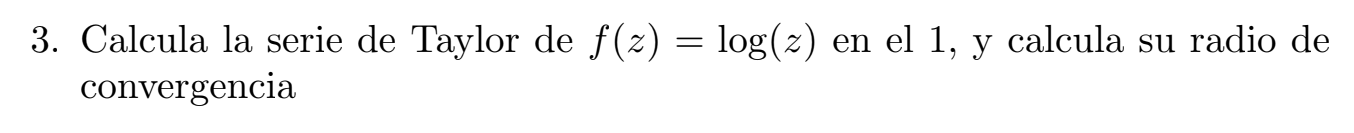
\includegraphics[width=0.8\linewidth]{3.png}
    \label{fig:enter-label}
\end{figure}

Usaré un método muy análogo al ejercicio anterior por lo que me iré más rápido, sin embargo, primero definiré al logatirmo. La función \( \log(z) \) es la rama principal del logaritmo natural en el plano complejo, definida como:
\[
\log(z) = \ln|z| + i\arg(z),
\]
donde \( \arg(z) \) pertenece al intervalo \( (-\pi, \pi] \). Consideramos \( \log(z) \) como una función holomorfa en el dominio \( \mathbb{C} \setminus (\mathbb{R^{+}})^{c} \), es decir, el plano complejo excluyendo el eje negativo real y el cero.
Para desarrollar la serie de Taylor de \( \log(z) \) alrededor de \( z = 1 \), consideramos \( w = z - 1 \), de modo que \( z = w + 1 \). Sustituyendo en la función:
\[
\log(z) = \log(1 + w).
\]

El desarrollo de \( \log(1+w) \) es conocido como la serie de Taylor estándar de \( \log(1+w) \), válida para \( |w| < 1 \):
\[
\log(1+w) = \sum_{n=1}^\infty (-1)^{n+1} \frac{w^n}{n}.
\]

Por lo tanto, tenemos:
\[
\log(z) = \sum_{n=1}^\infty (-1)^{n+1} \frac{(z-1)^n}{n}, \quad \text{para } |z-1| < 1.
\]

Esta es la serie de Taylor de \( \log(z) \) alrededor de \( z = 1 \). \\

El radio de convergencia de la serie de Taylor depende de la distancia desde el centro de expansión \( z = 1 \) hasta la singularidad más cercana de la función \( \log(z) \). 

La función \( \log(z) \) tiene una singularidad en \( z = 0 \), que está a una distancia \( |1-0| = 1 \) de \( z = 1 \). Por lo tanto, el radio de convergencia es:
\[
R = 1.
\]

La serie converge para \( |z-1| < 1 \), es decir, dentro del disco abierto centrado en \( z = 1 \) y de radio 1, algo que nuevamente ya esperábamos con solo ver el problema con el truquillo visto en clase, pues como hemos definido el logaritmo existe un "rayo singularidad" que si nos centramos en el 1 entonces podemos trazar una bola abierta de a lo más radio 1 sin indefinirse.

\begin{figure}[h]
    \centering
    
\includegraphics[width=0.75\linewidth]{4.png}
    \label{fig:enter-label}
\end{figure}
\begin{proof}
Sea \( f: U \to \mathbb{C} \) una función analítica en una región \( U \). Por la definición, \( f \) es una función holomorfa, lo que implica que es complejo diferenciable en \( U \) y además de clase $C^{\infty}$. Esto significa que \( f \) tiene una representación en series de potencias en torno a cada punto de \( U \). Alrededor de cualquier punto \( z_0 \in U \), la función \( f \) se puede expresar como:
   \[
   f(z) = \sum_{n=0}^\infty a_n (z - z_0)^n, \quad \text{donde } a_n = \frac{f^{(n)}(z_0)}{n!}.
   \]
   Si \( f(z_0) = 0 \), entonces \( a_0 = 0 \). Viz., si \( z_0 \) es un cero de \( f \), existe un entero \( m \geq 1 \) tal que:
   \[
   a_0 = a_1 = \cdots = a_{m-1} = 0 \quad \text{y} \quad a_m \neq 0.
   \]
   Entonces, \( f \) se puede escribir como:
   \[
   f(z) = (z - z_0)^m g(z),
   \]
   donde \( g(z) \) es analítica en \( U \) y \( g(z_0) \neq 0 \). Como \( g(z) \) es analítica y \( g(z_0) \neq 0 \), existe un entorno abierto \( V \subset U \) de \( z_0 \) tal que \( g(z) \neq 0 \) para todo \( z \in V \), en el entorno \( V \), \( f(z) = (z - z_0)^m g(z) \) implica que \( f(z) = 0 \) si y solo si \( z = z_0 \). Esto muestra que \( z_0 \) es un cero aislado de \( f \), ya que no hay otros ceros de \( f \) en \( V \).

$\therefore$ Dado que \( z_0 \) era un cero arbitrario de \( f \) y la demostración aplica a cualquier cero, se concluye que todos los ceros de \( f \) son aislados.
\end{proof}

\begin{figure}
    \centering
    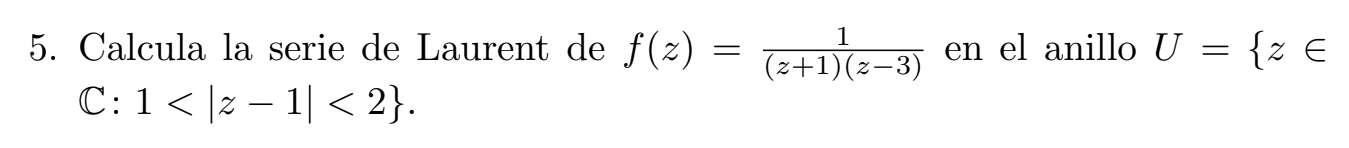
\includegraphics[width=0.8\linewidth]{5.png}
    \label{fig:enter-label}
\end{figure}

La función \( f(z) \) tiene dos singularidades: una en \( z = -1 \) y otra en \( z = 3 \). El anillo dado por \( U \) está centrado en \( z = 1 \), y satisface \( |z - 1| > 1 \) (excluyendo \( z = -1 \)) y \( |z - 1| < 2 \) (excluyendo \( z = 3 \)). Simplificamos usando fracciones parciales.
\[
\frac{1}{(z+1)(z-3)} = \frac{A}{z+1} + \frac{B}{z-3},
\]
multiplicamos por el denominador común \( (z+1)(z-3) \):
\[
1 = A(z-3) + B(z+1).
\]
Expandiendo:
\[
1 = A z - 3A + B z + B.
\]
Agrupando términos:
\[
1 = (A + B)z + (-3A + B).
\]
Igualamos coeficientes:
\begin{itemize}
    \item Para \( z \): \( A + B = 0 \),
    \item Término independiente: \( -3A + B = 1 \).
\end{itemize}

\noindent Resolviendo el sistema:
\begin{enumerate}
    
\item  De \( A + B = 0 \), tenemos \( B = -A \).
\item Sustituyendo en \( -3A + B = 1 \):
   \[
   -3A - A = 1 \implies -4A = 1 \implies A = -\frac{1}{4}.
   \]
\item Luego, \( B = -A = \frac{1}{4} \).
\end{enumerate}

Por lo tanto:
\[
\frac{1}{(z+1)(z-3)} = \frac{-1/4}{z+1} + \frac{1/4}{z-3}.
\]

Ahora sí, hacemos el desarrollo en series de Laurent.\\
(a) Primer término: \( \frac{-1/4}{z+1} \), reescribimos \( z+1 \) en términos de \( z-1 \):
\[
z+1 = (z-1) + 2.
\]
Por lo tanto:
\[
\frac{-1/4}{z+1} = \frac{-1/4}{(z-1) + 2}.
\]
Factorizamos \( 2 \) del denominador:
\[
\frac{-1/4}{z+1} = \frac{-1/4}{2} \cdot \frac{1}{1 + \frac{z-1}{2}} = -\frac{1}{8} \cdot \frac{1}{1 - \left(-\frac{z-1}{2}\right)}.
\]
Utilizando la expansión en serie geométrica para \( |z-1| > 1 \) (dado que \( |\frac{z-1}{2}| < 1 \)):
\[
\frac{1}{1 - \left(-\frac{z-1}{2}\right)} = \sum_{n=0}^\infty \left(-\frac{z-1}{2}\right)^n = \sum_{n=0}^\infty \frac{(-1)^n}{2^n} (z-1)^n.
\]
Entonces:
\[
\frac{-1/4}{z+1} = -\frac{1}{8} \sum_{n=0}^\infty \frac{(-1)^n}{2^n} (z-1)^n = \sum_{n=0}^\infty \frac{(-1)^{n+1}}{2^{n+3}} (z-1)^n.
\]

(b) Segundo término: \( \frac{1/4}{z-3} \), paralelamente reescribimos \( z-3 \) en términos de \( z-1 \):
\[
z-3 = (z-1) - 2.
\]
Por lo tanto:
\[
\frac{1/4}{z-3} = \frac{1/4}{(z-1) - 2}.
\]
Factorizamos \( z-1 \) en el denominador:
\[
\frac{1/4}{z-3} = \frac{1/4}{z-1} \cdot \frac{1}{1 - \frac{2}{z-1}}.
\]
Usando la expansión geométrica para \( |z-1| > 1 \) (ya que \( |\frac{2}{z-1}| < 1 \)):
\[
\frac{1}{1 - \frac{2}{z-1}} = \sum_{n=0}^\infty \left(\frac{2}{z-1}\right)^n.
\]
Por lo tanto:
\[
\frac{1/4}{z-3} = \frac{1/4}{z-1} \sum_{n=0}^\infty \frac{2^n}{(z-1)^n} = \sum_{n=0}^\infty \frac{2^n}{4} (z-1)^{-n-1}.
\]

Ahora solo sumamos ambos términos (a)+(b):
\begin{align*}
f(z) &= \sum_{n=0}^\infty \frac{(-1)^{n+1}}{2^{n+3}} (z-1)^n + \sum_{n=0}^\infty \frac{2^n}{4} (z-1)^{-n-1} \\
&= \sum_{n=0}^\infty \frac{(-1)^{n+1}}{2^{n+3}} (z-1)^n +  \frac{2^n}{4} (z-1)^{-n-1}.
\end{align*}

\begin{figure}[h]
    \centering
    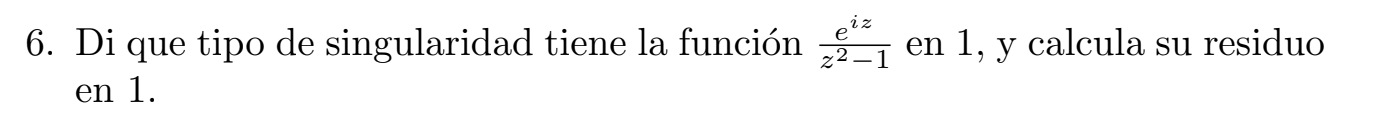
\includegraphics[width=0.8\linewidth]{6.png}
    \label{fig:enter-label}
\end{figure}
La función \( f(z) \) tiene un denominador \( z^2 - 1 \), que se factoriza como $(z - 1)(z + 1).$ Por lo tanto, \( f(z) \) tiene singularidades en los puntos \( z = 1 \) y \( z = -1 \).

Cerca de \( z = 1 \), podemos escribir \( f(z) \) como:
\[
f(z) = \frac{e^{iz}}{(z - 1)(z + 1)}.
\]
El término \( (z - 1) \) en el denominador indica que \( z = 1 \) es un polo simple, ya que el factor \( (z - 1) \) aparece con exponente 1 y no se cancela.\\

\noindent El residuo de \( f(z) \) en un polo simple \( z_0 \) se calcula como sigue:
\[
\text{Res}(f, z_0) = \lim_{z \to z_0} (z - z_0) f(z).
\]
En nuestro caso, \( z_0 = 1 \), por lo que:
\[
\text{Res}(f, 1) = \lim_{z \to 1} (z - 1) \frac{e^{iz}}{(z - 1)(z + 1)}.
\]
Simplificamos:
\[
\text{Res}(f, 1) = \lim_{z \to 1} \frac{e^{iz}}{z + 1}.
\]
Sustituyendo \( z = 1 \):
\[
\text{Res}(f, 1) = \frac{e^{i \cdot 1}}{1 + 1} = \frac{e^i}{2}.
\]
\newpage

\begin{figure}
    \centering
    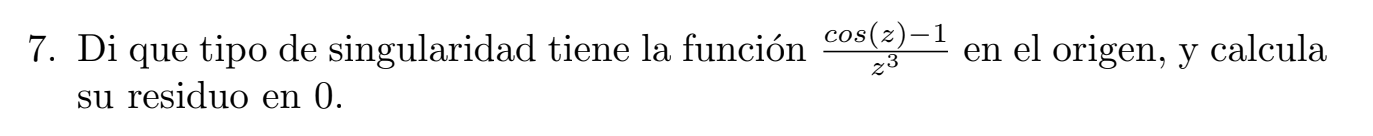
\includegraphics[width=0.8\linewidth]{7.png}
    \label{fig:enter-label}
\end{figure}

Para estudiar el comportamiento de \(f(z)\) cerca de \(z = 0\), desarrollamos el numerador \(\cos(z) - 1\) mediante la serie de Taylor de \(\cos(z)\) en torno a \(z = 0\):

\[
\cos(z) = 1 - \frac{z^2}{2!} + \frac{z^4}{4!} - \frac{z^6}{6!} + \cdots
\]

Por lo tanto,

\[
\cos(z) - 1 = -\frac{z^2}{2!} + \frac{z^4}{4!} - \frac{z^6}{6!} + \cdots = -\frac{z^2}{2} + \frac{z^4}{24} - \frac{z^6}{720} + \cdots
\]

Sustituyendo este desarrollo en \(f(z)\), obtenemos:

\[
f(z) = \frac{\cos(z) - 1}{z^3} = \frac{-\frac{z^2}{2} + \frac{z^4}{24} - \frac{z^6}{720} + \cdots}{z^3}.
\]

Simplificamos dividiendo cada término por \(z^3\):

\[
f(z) = -\frac{1}{2z} + \frac{z}{24} - \frac{z^3}{720} + \cdots
\]

Este desarrollo muestra que \(f(z)\) tiene un término principal proporcional a \(-\frac{1}{2z}\), que es singular en \(z = 0\). Por tanto, la singularidad en \(z = 0\) es un polo simple. El residuo de una función \(f(z)\) en un polo simple \(z = z_0\) como ya se ha comentado está dado por:

\[
 = \lim_{z \to z_0} \big((z - z_0)f(z)\big).
\]

En este caso, \(z_0 = 0\), y multiplicamos \(f(z)\) por \(z\):

\[
z f(z) = z \cdot \left(-\frac{1}{2z} + \frac{z}{24} - \frac{z^3}{720} + \cdots\right).
\]

Esto se reduce a:

\[
z f(z) = -\frac{1}{2} + \frac{z^2}{24} - \frac{z^4}{720} + \cdots
\]

Tomando el límite cuando \(z \to 0\), los términos que dependen de \(z\) desaparecen, y queda:

\[
\text{Res}(f,0) = -\frac{1}{2}.
\]

\begin{figure}[h]
    \centering
    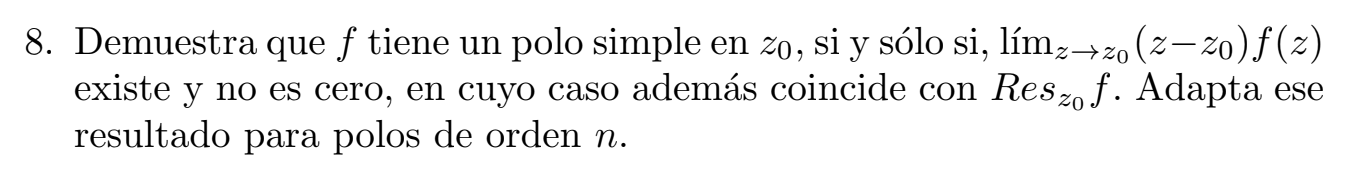
\includegraphics[width=0.8\linewidth]{8.png}
    \label{fig:enter-label}
\end{figure}

\begin{proof}
Sea \(f(z)\) una función meromorfa en un entorno de \(z_0\). Decimos que \(z_0\) es un polo simple de \(f(z)\) si \(f(z)\) puede escribirse como:

\[
f(z) = \frac{g(z)}{z - z_0},
\]

\noindent donde \(g(z)\) es holomorfa en \(z_0\) y \(g(z_0) \neq 0\).\\

$\longrightarrow )$\\

Se sigue que...\\
Si \(z_0\) es un polo simple, entonces \(\lim_{z \to z_0} (z - z_0)f(z)\) existe, no es cero, y coincide con el residuo\\
Si \(z_0\) es un polo simple, por la definición dada, tenemos:

\[
f(z) = \frac{g(z)}{z - z_0}.
\]

Multiplicamos ambos lados por \(z - z_0\):

\[
(z - z_0)f(z) = g(z).
\]

Ahora, evaluamos el límite cuando \(z \to z_0\). Como \(g(z)\) es holomorfa en \(z_0\), es continua en \(z_0\), y su límite existe y es:

\[
\lim_{z \to z_0} (z - z_0)f(z) = g(z_0).
\]

Dado que \(g(z_0) \neq 0\), el límite existe y no es cero.

Por otra parte, recordemos que el residuo de \(f(z)\) en \(z_0\) está dado por:

\[
\text{Res}_{z_0}f = \frac{1}{2\pi i} \int_{\gamma} f(z) \, dz,
\]

donde \(\gamma\) es un contorno cerrado alrededor de \(z_0\). Para un polo simple, esto equivale a:

\[
\text{Res}_{z_0}f = g(z_0),
\]

que es exactamente el mismo valor que \(\lim_{z \to z_0} (z - z_0)f(z)\). Por lo tanto, hemos demostrado la ida.\\

$\longleftarrow )$ \\

Si \(\lim_{z \to z_0} (z - z_0)f(z)\) existe, no es cero, entonces \(z_0\) es un polo simple, y el límite coincide con el residuo

Supongamos que \(\lim_{z \to z_0} (z - z_0)f(z) = L\), con \(L \neq 0\). Esto implica que podemos escribir:

\[
(z - z_0)f(z) = g(z),
\]

donde \(g(z)\) es holomorfa en un entorno de \(z_0\), pues el límite existe y \(g(z_0) = L\). Entonces,

\[
f(z) = \frac{g(z)}{z - z_0}.
\]

Esta es precisamente la forma que define un polo simple en \(z_0\). Además, el residuo en \(z_0\) es:

\[
\text{Res}_{z_0}f = g(z_0) = L = \lim_{z \to z_0} (z - z_0)f(z).
\]

Por lo tanto, el regreso ya también queda demostrado. \\

\dots \\

\textbf{Extensión a polos de orden \(n\)}

Decimos que \(z_0\) es un polo de orden \(n \geq 1\) de \(f(z)\) si \(f(z)\) puede escribirse como:

\[
f(z) = \frac{g(z)}{(z - z_0)^n},
\]

donde \(g(z)\) es holomorfa en \(z_0\) y \(g(z_0) \neq 0\). \\

Para un polo de orden \(n\), consideramos el límite generalizado:

\[
\lim_{z \to z_0} (z - z_0)^n f(z).
\]

Si \(f(z) = \frac{g(z)}{(z - z_0)^n}\), entonces:

\[
(z - z_0)^n f(z) = g(z).
\]

Como \(g(z)\) es holomorfa en \(z_0\), su límite existe y es \(g(z_0) \neq 0\). Por lo tanto:

\[
\lim_{z \to z_0} (z - z_0)^n f(z) = g(z_0).
\]

Además, sabemos que los residuos para polos de orden \(n\) se obtienen de la fórmula general:

\[
\text{Res}_{z_0}f = \frac{1}{(n-1)!} \lim_{z \to z_0} \frac{d^{n-1}}{dz^{n-1}}\big[(z - z_0)^n f(z)\big].
\]

En particular, cuando \(n = 1\) (polo simple), este resultado coincide con la demostración previa. Para \(n > 1\), la fórmula garantiza una extensión natural.
\end{proof}

\begin{figure}[h]
    \centering
    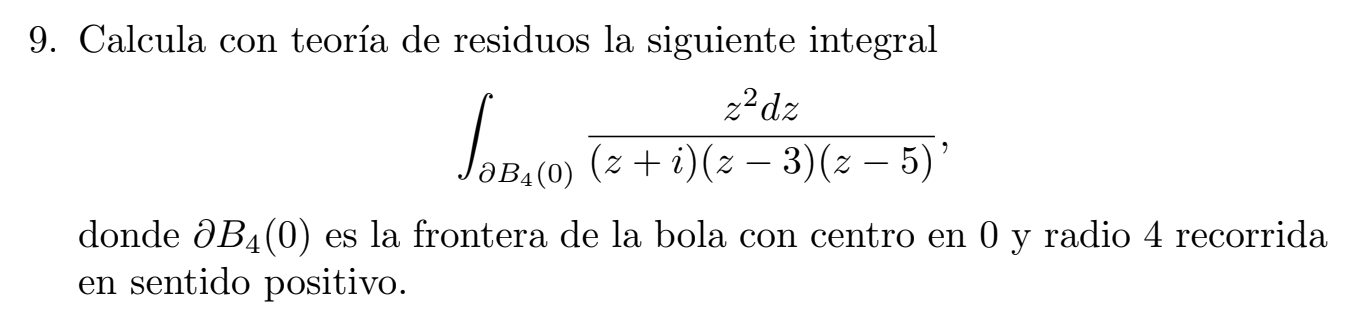
\includegraphics[width=0.7\linewidth]{9.png}
    \label{fig:enter-label}
\end{figure}

El integrando es:

\[
f(z) = \frac{z^2}{(z + i)(z - 3)(z - 5)}.
\]

Los polos de \(f(z)\) simplemente son los $z_i\in Domf$ tal que su imagen genera una indeterminación, directamente se ve que por las descomposición mónica del denominador son:

\[
z = -i, \quad z = 3, \quad z = 5.
\]

Sin embargo, el contorno de integración está restringido a \(\partial B_4(0)\), que corresponde al círculo centrado en \(z = 0\) con radio \(4\). De los polos identificados, solo los que están dentro de este círculo contribuyen a la integral. Estos son:

\[
z = -i \quad \text{y} \quad z = 3.
\]

El polo \(z = 5\) está fuera del contorno y no afecta el resultado. \\

Ahora podemos aplicar Teoría de Residuos, si \(f(z)\) es una función meromorfa en un dominio que contiene el contorno cerrado \(\gamma\), y \(z_1, z_2, \dots, z_k\) son las singularidades de \(f(z)\) dentro de \(\gamma\), entonces:

\[
\int_{\gamma} f(z) \, dz = 2\pi i \sum_{j=1}^k \text{Res}_{z = z_j} f.
\]

En nuestro caso, necesitamos calcular los residuos de \(f(z)\) en \(z = -i\) y \(z = 3\), y sumar sus contribuciones, recordando que en $z=5$ no nos importa obtener su residuo pues es un polo fuera del interior de $B_4(0)$.

El polo \(z = -i\) es un polo simple porque el factor \(z + i\) aparece linealmente en el denominador. El residuo en \(z = -i\) se calcula como:

\[
\text{Res}_{z = -i} f = \lim_{z \to -i} (z + i)f(z).
\]

Sustituyendo \(f(z)\), tenemos:

\[
(z + i)f(z) = (z + i) \cdot \frac{z^2}{(z + i)(z - 3)(z - 5)} = \frac{z^2}{(z - 3)(z - 5)}.
\]

Evaluando en \(z = -i\), obtenemos:

\[
\text{Res}_{z = -i} f = \frac{(-i)^2}{((-i) - 3)((-i) - 5)}.
\]

Simplificamos:

\[
(-i)^2 = -1, \quad (-i) - 3 = -i - 3, \quad (-i) - 5 = -i - 5.
\]

Por lo tanto:

\[
\text{Res}_{z = -i} f = \frac{-1}{(-i - 3)(-i - 5)}.
\]

Multiplicamos el denominador:

\[
(-i - 3)(-i - 5) = (-i - 3)(-i - 5) = (-i)^2 - 8i + 15 = -1 - 8i + 15 = 14 - 8i.
\]

Entonces:

\[
\text{Res}_{z = -i} f = \frac{-1}{14 - 8i}.
\]

El polo \(z = 3\) también es simple. El residuo en \(z = 3\) se calcula como:

\[
\text{Res}_{z = 3} f = \lim_{z \to 3} (z - 3)f(z).
\]

Sustituyendo \(f(z)\), tenemos:

\[
(z - 3)f(z) = (z - 3) \cdot \frac{z^2}{(z + i)(z - 3)(z - 5)} = \frac{z^2}{(z + i)(z - 5)}.
\]

Evaluando en \(z = 3\), obtenemos:

\[
\text{Res}_{z = 3} f = \frac{3^2}{(3 + i)(3 - 5)}.
\]

Simplificamos:

\[
3^2 = 9, \quad 3 + i = 3 + i, \quad 3 - 5 = -2.
\]

Por lo tanto:

\[
\text{Res}_{z = 3} f = \frac{9}{(3 + i)(-2)} = \frac{-9}{3 + i}.
\]

Ahora simplemente sumamos los residuos dentro del contorno:

\[
\int_{\partial B_4(0)} f(z) \, dz = 2\pi i \left( \text{Res}_{z = -i} f + \text{Res}_{z = 3} f \right).
\]

Sustituimos los valores calculados:\\

\noindent 1. \(\text{Res}_{z = -i} f = \frac{-1}{14 - 8i}\),\\
2. \(\text{Res}_{z = 3} f = \frac{-9}{3 + i}\). \\


\[
\therefore \int_{\partial B_4(0)} f(z) \, dz = 2\pi i \left( \frac{-1}{14 - 8i} + \frac{-9}{3 + i} \right).
\]

\begin{figure}[h]
    \centering
    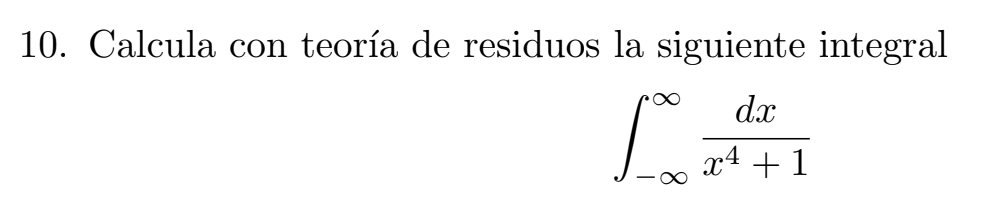
\includegraphics[width=0.6\linewidth]{10.png}
    \label{fig:enter-label}
\end{figure}

Para poder aplicar teoría de residuos descomponemos el denominador en polinomios mónicos, sin embargo es un poco extenso el proceso así que mejor primero obtendremos los polos. Véase que los valores para los que $x^4+1=0$ son los polos de esta función (si f(x) fuera una función que mapea complejos en complejos), sin embargo para todo x valor en el dominio de f jamás existirá mapeo al cero, pues el exponente de x es par, agréguese que siempre es cóncava por criterio de la segunda derivada, por lo que nos trasladamos al campo de los complejos extendidos, $f(x) :x \in \mathbb{R} \rightarrow \tilde{f}(z): z\in \mathbb{\hat{C}}$. Con esto me refiero a que $\forall z \in \hat{\mathbb{C}}: z=x, \tilde{f}(z) = f(x)$. Nuestra propuesta es $\tilde{f}(z)=\frac{1}{z^4+1}$, calculamos ahora sí los polos.

\begin{align*}
    z^4 &= -1 \\
    z_{k-1} &= e^{i(\pi/4 + k\pi/2)} : k\in \{1,2,3,4\} \\
    z_0 = e^{i(\pi/4)} = \cos(\pi/4) + i\sin(\pi/4) &= \frac{\sqrt{2}}{2} + i\frac{\sqrt{2}}{2} \\
    z_1 = e^{i(\pi/4 + \pi/2)} = e^{i(3\pi/4)} = \cos(3\pi/4) + i\sin(3\pi/4) &= -\frac{\sqrt{2}}{2} + i\frac{\sqrt{2}}{2} \\
    z_2 = e^{i(\pi/4 + \pi)} = e^{i(5\pi/4)} = \cos(5\pi/4) + i\sin(5\pi/4) &= -\frac{\sqrt{2}}{2} - i\frac{\sqrt{2}}{2} \\
     z_3 = e^{i(\pi/4 + 3\pi/2)} = e^{i(7\pi/4)} = \cos(7\pi/4) + i\sin(7\pi/4) &= \frac{\sqrt{2}}{2} - i\frac{\sqrt{2}}{2} 
\end{align*}

Ahora que tenemos los polos, podemos identificar cuáles están en el semiplano superior, ya que solo esos contribuyen al residuo cuando integramos sobre un contorno semicircular en el semiplano superior. De las raíces calculadas, los polos en el semiplano superior son aquellos con parte imaginaria positiva, las únicas que cumplen esto son $z_0, \,z_1$.\\

Ahora sí podemos utilizar teoría de los residuos.

\[
\int_{\gamma} f(z) \, dz = 2\pi i \sum_{j=1}^k \text{Res}_{z = z_j} f.
\]

Nótese que las raíces $z_k$ son la descomposición en polinomios mónicos de $z^4+1$, i.e.

$$ z^4+1 = \prod_{k=0}^{3} (z-z_k) $$

Entonces por teorema de fracciones parciales es facil ver que $z_k$ son polos de $\tilde{f}$. Es decir, la forma de sacar los residuos requeridos es como sigue:

\[
\text{Res}(f, z_0) = \lim_{z \to z_0} \frac{z - z_0}{z^4 + 1} = \lim_{z \to z_0} \frac{1}{(z - z_1)(z - z_2)(z - z_3)}
\]

Para \( z_0 = \frac{\sqrt{2}}{2} + i\frac{\sqrt{2}}{2} \) el residuo es:
\[
\text{Res}(f, z_0) = \lim_{z \to z_0} \frac{1}{(z_0 - z_1)(z_0 - z_2)(z_0 - z_3)}
\]

De donde
\[
z_0 - z_1 = \sqrt{2}
\]
\[
z_0 - z_2 = \sqrt{2} + i\sqrt{2}
\]
\[
z_0 - z_3 = i\sqrt{2}
\]

\[
\Rightarrow \text{Res}(f, z_0) = \frac{1}{\sqrt{2}(\sqrt{2} + i\sqrt{2})(i\sqrt{2})}
\]

Para \( z_1 = -\frac{\sqrt{2}}{2} + i\frac{\sqrt{2}}{2} \) es análogo.

\[
\text{Res}(f, z_1) = \frac{1}{(z_1 - z_0)(z_1 - z_2)(z_1 - z_3)}
\]

De donde
\[
z_1 - z_0 = -\sqrt{2}
\]
\[
z_1 - z_2 = i\sqrt{2}
\]
\[
z_1 - z_3 = \sqrt{2} + i\sqrt{2}
\]
\[
\Rightarrow \text{Res}(f, z_1) = \frac{1}{(-\sqrt{2})(i\sqrt{2})(\sqrt{2} + i\sqrt{2})}
\]

\begin{equation*}
    \int_{-\infty}^{\infty} \frac{d x}{x^{4}+1} = 2\pi i \left( \text{Res}(f, z_0) + \text{Res}(f, z_1) \right) = 2\pi i \left( \frac{1}{\sqrt{2}(\sqrt{2} + i\sqrt{2})(i\sqrt{2} )} + \frac{1}{(-\sqrt{2})(i\sqrt{2})(\sqrt{2} + i\sqrt{2})}     \right)
\end{equation*}

Algo hice mal no tenía que dar cero aaaaaaaaaaaaaaaaaaaaaaaaaaaaaaaaaaaaaaaaaaaaaaaaaaaaaaaaaaaaaaaa 



\end{document}



